\chapter{Getting Started}

Most UI elements can be interacted with by left clicking (select), left dragging (move), using the scroll wheel (zoom),
double clicking (open properties dialog), or right clicking (context menu).

%If you have a multi-button gaming mouse, button 8 stops the trigger and button 9 starts. These bindings are not
%currently configurable.

Most text fields allow SI prefixes for scaling values (mV, us, GHz, etc).

\section{Documentation Conventions}

Items to be selected from a menu are displayed in \menustyle{monospace font}.

Multilevel menu paths are separated by a / character. For example, \menustyle{Attenuation / 1x} means to open the
\menustyle{Attenuation} submenu and select the \menustyle{1x} item.

If there are multiple options for a menu or configuration option, they are displayed in square brackets and separated
by a | character. For example, \menustyle{Move waveform to / Waveform Group [1|2]} means to select either
\menustyle{Waveform Group 1} or \menustyle{Waveform Group 2} from the \menustyle{Move waveform to}
menu.

This project is under active development and is not anywhere near feature complete! As a result, this document is
likely to refer to active bug or feature request tickets on the GitHub issue trackers. Issues are referenced as
repository:ticket, for example \issue{scopehal-apps}{3}.

\section{Host System Requirements}

The majority of development is performed on Linux operating systems (primarily Debian and Arch) so this is the most well
tested platform, however Windows and Mac OS are also supported.

Any 64-bit Intel or AMD processor, or Apple Silicon Mac, should be able to run ngscopeclient. If AVX2 and/or AVX512F
support is present ngscopeclient will use special optimized versions of some signal processing functions, however
neither instruction set is required. Other (non Apple Silicon) ARM64 platforms may work if a compatible GPU is
available, but have not been tested. 32-bit platforms are not supported due to the significant RAM requirements.

A mouse with scroll wheel, or touchpad with scroll gesture support, is mandatory to enable full use of the UI. We may
explore alternative input methods for some UI elements in the future.

Any GPU with Vulkan support should be able to run ngscopeclient, however Vulkan 1.2 will deliver better performance.
The minimum supported GPUs are:
\begin{itemize}
\item AMD: GCN based (Radeon HD 7000 and newer, January 2012)
\item Apple: all Apple Silicon devices (M1 and newer)
\item Intel: Iris Plus 540 or HD Graphics 520 (Skylake, August 2015)
\item NVIDIA: Maxwell architecture (GeForce GTX 700 series and newer, February 2014)
\end{itemize}

The minimum RAM requirement to actually launch ngscopeclient is relatively small, however actual memory consumption is
heavily dependent on workload and can easily reach into the tens of gigabytes when doing complex analysis on many
channels with deep history.

Typical RAM consumption examples:
\begin{itemize}
\item Default configuration with demo scope (4 channels 100K points, 10 waveforms of history, no analysis): 250 MB
\item 4M point live streaming with 10 waveforms of history, eye pattern, 8B/10B decode, and jitter histogram: 650 MB
\item Single 512M point waveform, no analysis or history: 2.1 GB
\item 512M point P/N channel waveforms with CDR and eye pattern, no history: 8.3 GB
\end{itemize}

Large amounts of GPU RAM are required for working with deep waveforms, especially if you intend to perform
complex analysis on them. Analog waveforms are stored in 32-bit floating point format internally, so a single 256
megapoint waveform will consume 1GB of GPU memory. Intermediate results in multi-step filter pipelines require GPU
memory as well, even if not displayed.

\section{Instrument Support}

ngscopeclient uses the libscopehal library to communicate with instruments, so any libscopehal-compatible hardware
should work with ngscopeclient. See the \hyperref[sec:scope-drivers]{Oscilloscope Drivers} section for more details on
which hardware is supported and how to configure specific drivers.

\section{Compilation}

ngscopeclient can be compiled on Linux, macOS, and Windows, but the specific steps that have to be taken differ quite a
lot between these the three.

TODO: rewrite and simplify this section once glscopeclient is deprecated and we've removed all remaining vestiges of
GTK dependencies

TODO: update URLs for most recent tested Vulkan SDK revision

\subsection{Linux}
\begin{enumerate}

\item Install dependencies.

On Debian/Ubuntu:

\begin{lstlisting}[language=sh, numbers=none]
sudo apt install build-essential cmake pkg-config libglm-dev \
	libgtkmm-3.0-dev libsigc++-2.0-dev libyaml-cpp-dev \
	liblxi-dev texlive texlive-fonts-extra libglew-dev \
	catch2 libvulkan-dev glslang-dev libglfw3-dev
\end{lstlisting}

On Fedora(this section is out of date):

\begin{lstlisting}[language=sh, numbers=none]
sudo dnf install gtkmm30-devel cmake pkg-config glm-devel \
	texlive libyaml-devel yaml-cpp-devel glew-devel \
	catch-devel vulkan-devel
\end{lstlisting}

If you are using an older stable release (such as Debian Buster), you may need to install catch2 from source
(https://github.com/catchorg/Catch2). Alternatively, you may pass -DBUILD\_TESTING=OFF to CMake to disable unit testing.

\item Install FFTS library:

\begin{lstlisting}[language=sh, numbers=none]
cd ~
git clone https://github.com/anthonix/ffts.git
cd ffts
mkdir build
cd build
cmake .. -DENABLE_SHARED=ON -DCMAKE_INSTALL_PREFIX=/usr
make -j4
sudo make install
\end{lstlisting}

\item Install Vulkan SDK:

\begin{lstlisting}[language=sh, numbers=none]
cd ~
mkdir vulkan
cd vulkan
wget https://sdk.lunarg.com/sdk/download/1.3.224.1/linux/vulkansdk-linux-x86_64-1.3.224.1.tar.gz
tar xf vulkansdk-linux-x86_64-1.3.224.1.tar.gz
rm -f vulkansdk-linux-x86_64-1.3.224.1.tar.gz
export VULKAN_SDK=~/vulkan/1.3.224.1/x86_64
sudo cp -r $VULKAN_SDK/include/vulkan/ /usr/local/include/
sudo cp -P $VULKAN_SDK/lib/libvulkan.so* /usr/local/lib/
sudo cp $VULKAN_SDK/lib/libVkLayer_*.so /usr/local/lib/
sudo mkdir -p /usr/local/share/vulkan/explicit_layer.d
sudo cp $VULKAN_SDK/etc/vulkan/explicit_layer.d/VkLayer_*.json /usr/local/share/vulkan/explicit_layer.d
sudo ldconfig
\end{lstlisting}

\item Build scopehal and scopehal-apps:

\begin{lstlisting}[language=sh, numbers=none]
export VULKAN_SDK=~/vulkan/1.3.224.1/x86_64
export PATH=$VULKAN_SDK/bin:$PATH
export LD_LIBRARY_PATH=$VULKAN_SDK/lib${LD_LIBRARY_PATH:+:$LD_LIBRARY_PATH}
export VK_LAYER_PATH=$VULKAN_SDK/etc/vulkan/explicit_layer.d

cd ~
git clone -{}-recursive https://github.com/ngscopeclient/scopehal-apps.git
cd scopehal-apps
mkdir build
cd build
cmake ../ -DCMAKE_BUILD_TYPE=Release -DCMAKE_INSTALL_PREFIX=/usr
make -j4
\end{lstlisting}

\item Install scopehal and scopehal-apps:

\begin{lstlisting}[language=sh, numbers=none]
cd ~/scopehal-apps/build
sudo make install
\end{lstlisting}

\end{enumerate}

\subsection{macOS}
\begin{enumerate}

\item Install dependencies.

With Homebrew (\href{https://brew.sh}{brew.sh}):

\begin{lstlisting}[language=sh, numbers=none]
brew install pkg-config gtk+3 gtkmm3 glfw cmake yaml-cpp glew catch2 libomp
\end{lstlisting}

\item Install Vulkan SDK:

Download and install the Vulkan SDK from \href{https://sdk.lunarg.com/sdk/download/1.3.231.1/mac/vulkansdk-macos-1.3.231.1.dmg}{sdk.lunarg.com/sdk/download/1.3.231.1/mac/vulkansdk-macos-1.3.231.1.dmg}.

\item Build scopehal and scopehal-apps:

\begin{lstlisting}[language=sh, numbers=none]
export VULKAN_SDK=~/VulkanSDK/1.3.231.1/macOS
export PATH=${PATH}:${VULKAN_SDK}/bin:/opt/homebrew/bin
cd ~
git clone -{}-recursive https://github.com/ngscopeclient/scopehal-apps.git
cd scopehal-apps
mkdir build
cd build
cmake ../ -DCMAKE_BUILD_TYPE=Release -DCMAKE_INSTALL_PREFIX=/usr -DCMAKE_PREFIX_PATH="/opt/homebrew;/opt/homebrew/opt/libomp"
make -j4
\end{lstlisting}

\item Install scopehal and scopehal-apps:

Installation on macOS is not yet complete.
The binaries can be found in the build directory, such as ngscopeclient in \$HOME/scopehal-apps/build/src/ngscopeclient.

\end{enumerate}

\subsection{Windows}

On Windows, we make use of the MSYS2 development environment, which gives us access to the MingGW-w64 toolchain.
Since this toolchain allows ngscopeclient to be compiled as a native Windows application, the project might be run
outside of MSYS2.

\subsubsection{Installing from the package manager}

\begin{lstlisting}[language=sh, numbers=none]
pacman -Sy
pacman -S mingw-w64-x86_64-scopehal-apps
\end{lstlisting}

See also \href{https://packages.msys2.org/group/mingw-w64-x86_64-eda}{\lstinline{mingw-w64-x86_64-eda}}.

\subsubsection{Building from source}

\begin{enumerate}

\item Download and install MSYS2. You can download it from \href{https://www.msys2.org/}{msys2.org} or \href{https://github.com/msys2/msys2-installer/releases}{github.com/msys2/msys2-installer/releases}\\
It is of utmost importance that \textbf{all} steps outlined on the website are followed precisely, even if they might
seem unnecessary.
This will avoid lots of hard to diagnose problems later on in the build.\\

All following steps are to be done in a MinGW64 shell (\textbf{not} in a MSYS, MINGW32, CLANG64, CLANG32 or UCRT64 shell,
which also get installed by the MSYS2 installer).

\item Install WiX Toolset v3.11 (required to build the Windows x64 MSI)
You shall download and install WiX Toolset v3.11 in \begin{verbatim}C:\Program Files (x86)\WiX Toolset v3.11\end{verbatim}
https://wixtoolset.org/docs/wix3/

\item Install git and the toolchain:

\begin{lstlisting}[language=sh, numbers=none]
pacman -S git wget mingw-w64-x86_64-cmake mingw-w64-x86_64-toolchain
\end{lstlisting}

\item Build glslang tags/sdk-1.3.224.1:

Launch MSYS2 or MINGW64 as Administrator only for this step (it is mandatory to do the install in default path C:\\VulkanSDK ...)
\begin{lstlisting}[language=sh, numbers=none]
# Windows mingw64 glslang build (as it is not fully integrated in VulkanSDK-1.3.224.1 for Windows and built with Visual Studio 2017)
cd ~
git clone https://github.com/KhronosGroup/glslang.git
cd glslang
git checkout tags/sdk-1.3.224.1
git clone https://github.com/google/googletest.git External/googletest
cd External/googletest
git checkout 0c400f67fcf305869c5fb113dd296eca266c9725
cd ../..
./update_glslang_sources.py

SOURCE_DIR=~/glslang
BUILD_DIR=$SOURCE_DIR/build
mkdir -p $BUILD_DIR
cd $BUILD_DIR
cmake -DCMAKE_BUILD_TYPE=Release -G"MinGW Makefiles" $SOURCE_DIR -DCMAKE_INSTALL_PREFIX="$(pwd)/install"
cmake -{}-build . -{}-config Release -{}-target install
\end{lstlisting}

\item Install Vulkan SDK:

Launch MSYS2 or MINGW64 as Administrator only for this step (it is mandatory to do the install in default path C:\\VulkanSDK ...)
\begin{lstlisting}[language=sh, numbers=none]
cd ~
wget https://sdk.lunarg.com/sdk/download/1.3.224.1/windows/VulkanSDK-1.3.224.1-Installer.exe
./VulkanSDK-1.3.224.1-Installer.exe -{}-accept-licenses -{}-default-answer -{}-confirm-command install
rm -f VulkanSDK-1.3.224.1-Installer.exe
\end{lstlisting}

\item Check out the code

\begin{lstlisting}[language=sh, numbers=none]
cd ~
git clone -{}-recursive https://github.com/ngscopeclient/scopehal-apps
\end{lstlisting}

\item Execute makepkg-mingw in subdir MSYS2:

\begin{lstlisting}[language=sh, numbers=none]
cd ~/scopehal-apps/msys2
export VK_SDK_PATH=/c/VulkanSDK/1.3.224.1
export PATH=$VK_SDK_PATH/Bin:$PATH
export VULKAN_SDK=$VK_SDK_PATH
export GLSLANG_BUILD_PATH=~/glslang/build/install

MINGW_ARCH=mingw64 makepkg-mingw -{}-noconfirm -{}-noprogressbar -sCLf
\end{lstlisting}

The unit tests will not be run as part of this build - if you would like to run them, you will need to provide catch2
(https://github.com/catchorg/Catch2), and remove the -DBUILD\_TESTING=OFF flag from the PKGBUILD recipe in subdir
msys2.

\item Installing, copying binaries and running ngscopeclient.

Since ngscopeclient is built using the MinGW toolchain, it depends on a rather large number of dynamic libraries.
The recommended procedure is to install the package generated by makepkg-mingw on a MinGW64 shell:

\begin{lstlisting}[language=sh, numbers=none]
cd ~
cd msys2
pacman -U *.zst
\end{lstlisting}

This is equivalent to the package installed through \lstinline{pacman -S}, but it's built from the checked out commit,
instead of the pinned version available from MSYS2 repositories.

The \lstinline{*.zst} package includes metadata about the dependencies.
Therefore, when installed through \lstinline{pacman}, those will be installed automatically.
However, some users might want to use ngscopeclient outside of MSYS2.
In those cases, it needs to be installed first, and then a tarball/zipfile can be created by collecting all the dependencies.
This last approach is not officially supported yet.

\end{enumerate}

\section{Running ngscopeclient}

When running ngscopeclient with no arguments, an empty session (Fig. \ref{empty-window}) is created. To perform useful
work, you can:
\begin{itemize}
\item Open a saved session and reconnect to the instruments (\menustyle{File | Open Online})
\item Open a saved session without reconnecting to the instruments (\menustyle{File | Open Offline})
\item Open a recently used session (\menustyle{File | Recent Files})
\item Import waveforms from a third party file format(\menustyle{Add | Import})
\item Connect to an instrument (\menustyle{Add | Oscilloscope}, \menustyle{Add | Multimeter}, etc.)
\item Generate a synthetic waveform (\menustyle{Add | Generate})
\end{itemize}

\begin{figure}[h]
\centering
	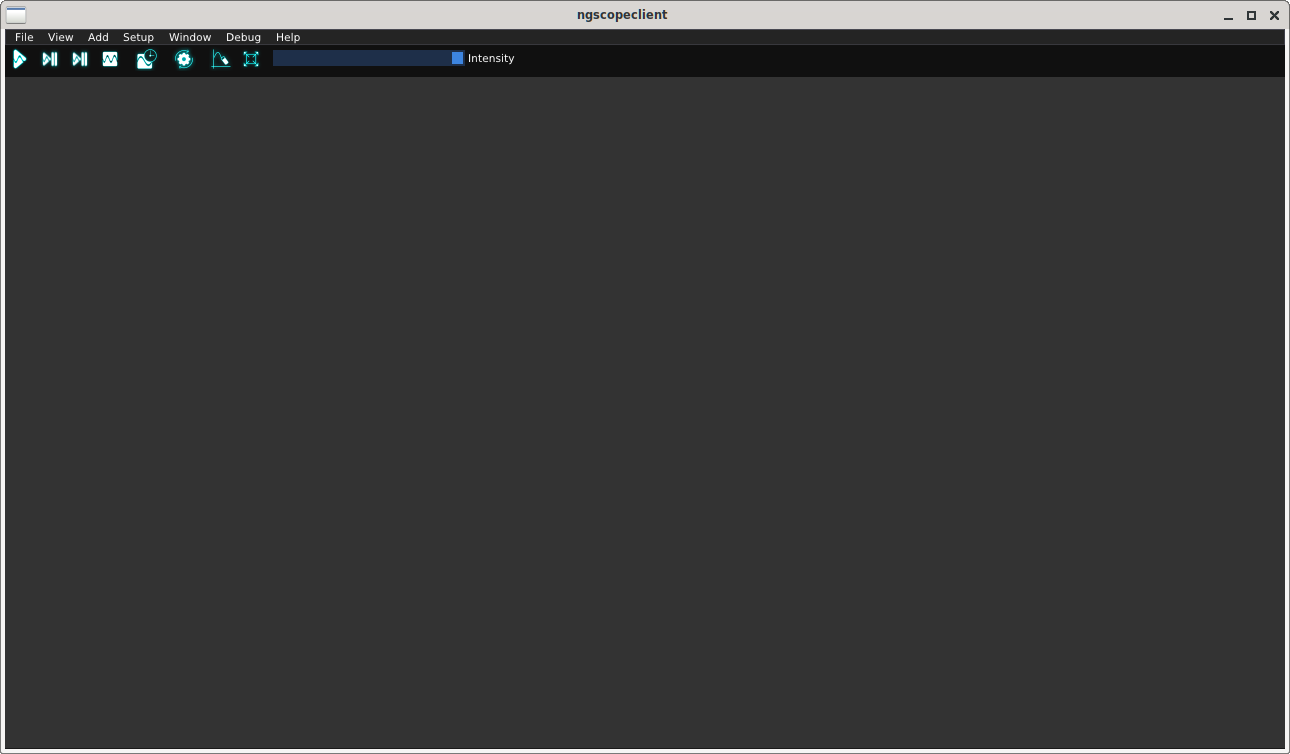
\includegraphics[width=12cm]{ng-images/empty-window.png}
\caption{Empty ngscopeclient session}
\label{empty-window}
\end{figure}

% TODO: add this section once these are implemented
\begin{comment}

\subsection{Configuration arguments}

Most of these arguments are intended for developers, but they can help troubleshoot unusual bugs.

\begin{itemize}

\item \texttt{-{}-noavx2}\\
Do not use AVX2 vector optimizations even if the CPU supports it.

\item \texttt{-{}-noavx512f}\\
Do not use AVX512F vector optimizations even if the CPU supports it.

\item \texttt{-{}-noglint64}\\
Do not use \texttt{GL\_ARB\_gpu\_shader\_int64} even if the GPU supports it.

\item \texttt{-{}-nogpufilter}\\
Do not use Vulkan (GPU accelerated) implementations of filter blocks, revert to software fallback.

\end{itemize}

\end{comment}

\subsection{Console verbosity arguments}

ngscopeclient takes standard liblogtools arguments for controlling console debug verbosity.

If no verbosity level is specified, the default is ``notice" (3). (We suggest using \texttt{-{}-debug} for routine use
until the v1.0 release to aid in troubleshooting.)

\begin{itemize}

\item \texttt{-{}-debug}\\
Sets the verbosity level to ``debug" (5).

\item \texttt{-l [file]}, \texttt{-{}-logfile [file]}\\
Writes a copy of all log messages to \texttt{file}. This is preferred over simply redirecting output with pipes, as
console escape sequences are stripped from the file log output.

\item \texttt{-L [file]}, \texttt{-{}-logfile-lines [file]}\\
Same as \texttt{-{}-logfile} except line buffering is turned on.

\item \texttt{-q}, \texttt{-{}-quiet}\\
Reduces the verbosity level by one. Can be specified more than once to lower verbosity by several steps.

\item \texttt{-{}-trace [class]}, \texttt{-{}-trace [class::function]} \\
Enables extra debug output from the class \texttt{class} or the function \texttt{class::function}. Has no effect unless
\texttt{-{}-debug} is also specified.

\item \texttt{-{}-stdout-only}\\
Sends all logging output to stdout. By default, error (level 1) and warning (level 2) messages go to stderr.

\item \texttt{-{}-verbose}\\
Sets the verbosity level to ``verbose" (4).

\end{itemize}

% TODO: add this section once these are implemented
\begin{comment}
\subsection{File arguments}
\label{import}

The file extension is used to determine the format. File extensions are case sensitive and must be lowercase to be
correctly interpreted.

\begin{itemize}
\item \texttt{[file.scopesession]}
Loads a saved session.

\item \texttt{[file.bin]} \\
Imports waveform data from the binary format used by Agilent, Keysight, and Rigol oscilloscopes.

\item \texttt{[file.complex]} \\
Imports complex I/Q data from a file. The file must contain interleaved (I, Q) pairs in either 8-bit signed/unsigned
integer, 16-bit signed integer, 32-bit normalized floating point, or 64-bit normalized floating point format.

The default format is 8 bit signed integer and may be changed from the filter graph editor or channel properties dialog
once the file is loaded. There is currently no way to specify other formats on the command line.

\item \texttt{[file.csv]} \\
Imports sample data from a CSV (comma-separated-value) file. More than one CSV file can be loaded at once (displayed as
separate points in history) by specifying multiple file names as long as they have identical column schemas.

Lines starting with a '\#' character are treated as comments and generally ignored by the parser. (If the comment format
matches that used by Digilent's WaveForms utility, timestamps and other metadata are extracted from the comments.)

If the first row of the CSV contains non-numeric characters, it is treated as a header row. Header content in the
timestamp column is ignored; headers in other columns are used as channel names in the imported waveform.

The first column of the CSV must contain sample timestamps, in seconds. Scientific notation is supported. Timestamps
must be monotonic (each row must have a timestamp strictly greater than that of the previous row).

ngscopeclient uses a heuristic to detect uniformly sampled waveforms, which enabled certain optimizations for display
and signal processing. If the standard deviation of intervals between samples is less than 1\% of the average sample
interval, the waveform is assumed to be uniformly sampled and timestamps are rounded to the nearest multiple of the
average interval. If the deviation is greater, the waveform is assumed to be sparsely sampled and timestamps are not
modified.

\item \texttt{[file.trc]} \\
Imports waveform data from a Teledyne LeCroy .trc binary waveform file.

\item \texttt{[file.vcd]} \\
Imports digital waveform data from a VCD (value change dump) file, typically created by a logic analyzer or HDL
simulator.

\item \texttt{[file.wav]} \\
Imports sample data from a WAV file.

\item \texttt{[file.wfm]} \\
Imports sample data from a Tektronix .wfm file. This import filter is still experimental and may not support all
features of the .wfm file format yet. If you have trouble importing some .wfm files please file a ticket on GitHub.

%%%%%%%%%%%%%%%%%%%%%%%%%%%%%%%%%%%%%%%%

\item \texttt{-{}-nodata}\\
When loading a .scopesession file, load settings only and not saved waveform data.

\item \texttt{-{}-reconnect}\\
When loading a .scopesession file, reconnect to the instrument and resume remote control. Current instrument settings
are overwritten with the configuration from the saved session.

\item \texttt{-{}-retrigger}\\
When loading a .scopesession file, arm the trigger immediately. has no effect unless \texttt{-{}-reconnect} is also
specified.

\end{itemize}

\subsection{Instrument arguments}

Example:
\begin{lstlisting}[language=sh, numbers=none]
./ngscopeclient -{}-debug \
	mylecroy:lecroy:vicp:myscope.example.com:1234 \
	myrigol:rigol:lan:rigol.example.com
\end{lstlisting}

\begin{itemize}
\item \texttt{[connection string]} \\
Connects to the specified instrument. By default, all channels are enabled and displayed.

\end{itemize}

Each instrument is described by a ``connection string" containing four colon-separated fields.

\begin{itemize}
\item Nickname. This can be any text string not containing spaces or colons. If you have only one instrument it's
largely ignored, but when multiple instruments are present channel names in the UI are prefixed with the nickname to
avoid ambiguity.
\item Driver name. This is a string identifying the command protocol the scope uses. Note that not all
scopes from the same vendor will use the same command set or driver!
\item Transport. This is is a string describing how the driver connects to the scope (e.g. RS232 or Ethernet)
\item Arguments for the driver identifying the device to connect to, separated by colons. This varies by driver but is
typically a hostname:port combination, TTY device path, or similar.
\end{itemize}

\end{comment}
